\chapter{Delivery}
\label{delivery}

With each of our core components now in place, this final chapter hopes to draw all the individual pieces together, along with discussing how they have been made available.

\section{Sentiment analysis engine}

Our sentiment analysis engine is brought together through the singleton \emph{Engine} class. This class initialises each of our three classifiers along with our topic extraction engine. Once initialised, status objects can be classified by calling its \texttt{classify(status)} method, which will return a hashmap containing each of the classifiers' results along with the status' topics, as demonstrated in listing \ref{delivery:classify_results}. The method can handle both \emph{Status} objects and \emph{Strings}.

\begin{lstlisting}[language=Ruby, caption={Returned part of speech tags for \emph{Example 1}}, label=delivery:classify_results]
# let status = Example 1
Engine.classify status
	=>
		{
			:subjective => true,
			:polarity => :positive,
			:emotion => [:trust],
			:topics => ["David Cameron", "job", "leader", "coalition", "labour"]
		}
\end{lstlisting}

Along with returning the results, the hashmap is written as JSON to the status' \texttt{classified\_status} attribute. Thus the above output is persisted in MongoDB and is referred to from that point forward whenever the status' classification is requested.

When the engine is running, it sets the \emph{TwitterStreaming} API to run in the background, constantly feeding data into MongoDB. Our sentiment engine polls this is every 10 seconds checking for new unclassified statuses, and if found it will syphon them off to the \texttt{classify(status)} method.

\section{Online API}

In order for us and others to make use of our collected and classified data, we offer two core web services. Our first, a classification service, is based upon our \emph{Engine} class. The second, a retrieval service, is built upon our MongoDB store. The web services are made available using the \emph{Sinatra} web framework. Below, is a more detailed outline of each service:

\begin{description}
	\item [\texttt{/classify?text=:string}] - when passed a status' textual content, this method will utilise the \emph{Engine} class in order to classify it. The text is formatted as a String object, and passed to the \texttt{classify(status)} method. The returned hashmap is formatted as JSON and delivered back to the user.
	\item [\texttt{/results/:params}] - allows the user to query our MongoDB store for classified statuses. With no parameters, the method will simply return the last 200 classified statuses. With parameters, the user can specify \texttt{from} and \texttt{until} dates to retriever statuses from within a certain time frame. Additionally, the \texttt{subjective}, \texttt{polarity}, \texttt{emotion} and \texttt{topic} parameters each take a comma separated list of acceptable values. For example, 
	\begin{center}
		\texttt{polarity=positive\&topic=David\%20Cameron,NHS} 
	\end{center}
will return all positive statuses regarding David Cameron and the NHS. The results are formatted as a JSON array and returned to the user.
\end{description}

\section{Visualisation}

Our HTML5 visualisation utilises the \texttt{results} service above to render an interactive demonstration of sentiment on Twitter. Making use of the \emph{canvas} element, topics are rendered as spheres whose size grows as the number of statuses discussing them increases. Spheres whose topics tend to be discussed together are grouped closed to one another. The colour of the spheres is determined by their polarity and emotion. Using Plutchik's emotion wheel, topic spheres are rendered as in figure \ref{fig:visualisation}.

\begin{figure}
	\caption{Example demonstrating our visualisation's spheres and approach to emotion colouring. The labels inside each sphere would typically be a topic, however for the purpose of explanation, we have used the sphere's corresponding emotion label instead.}
	\label{fig:visualisation}
	\centering
		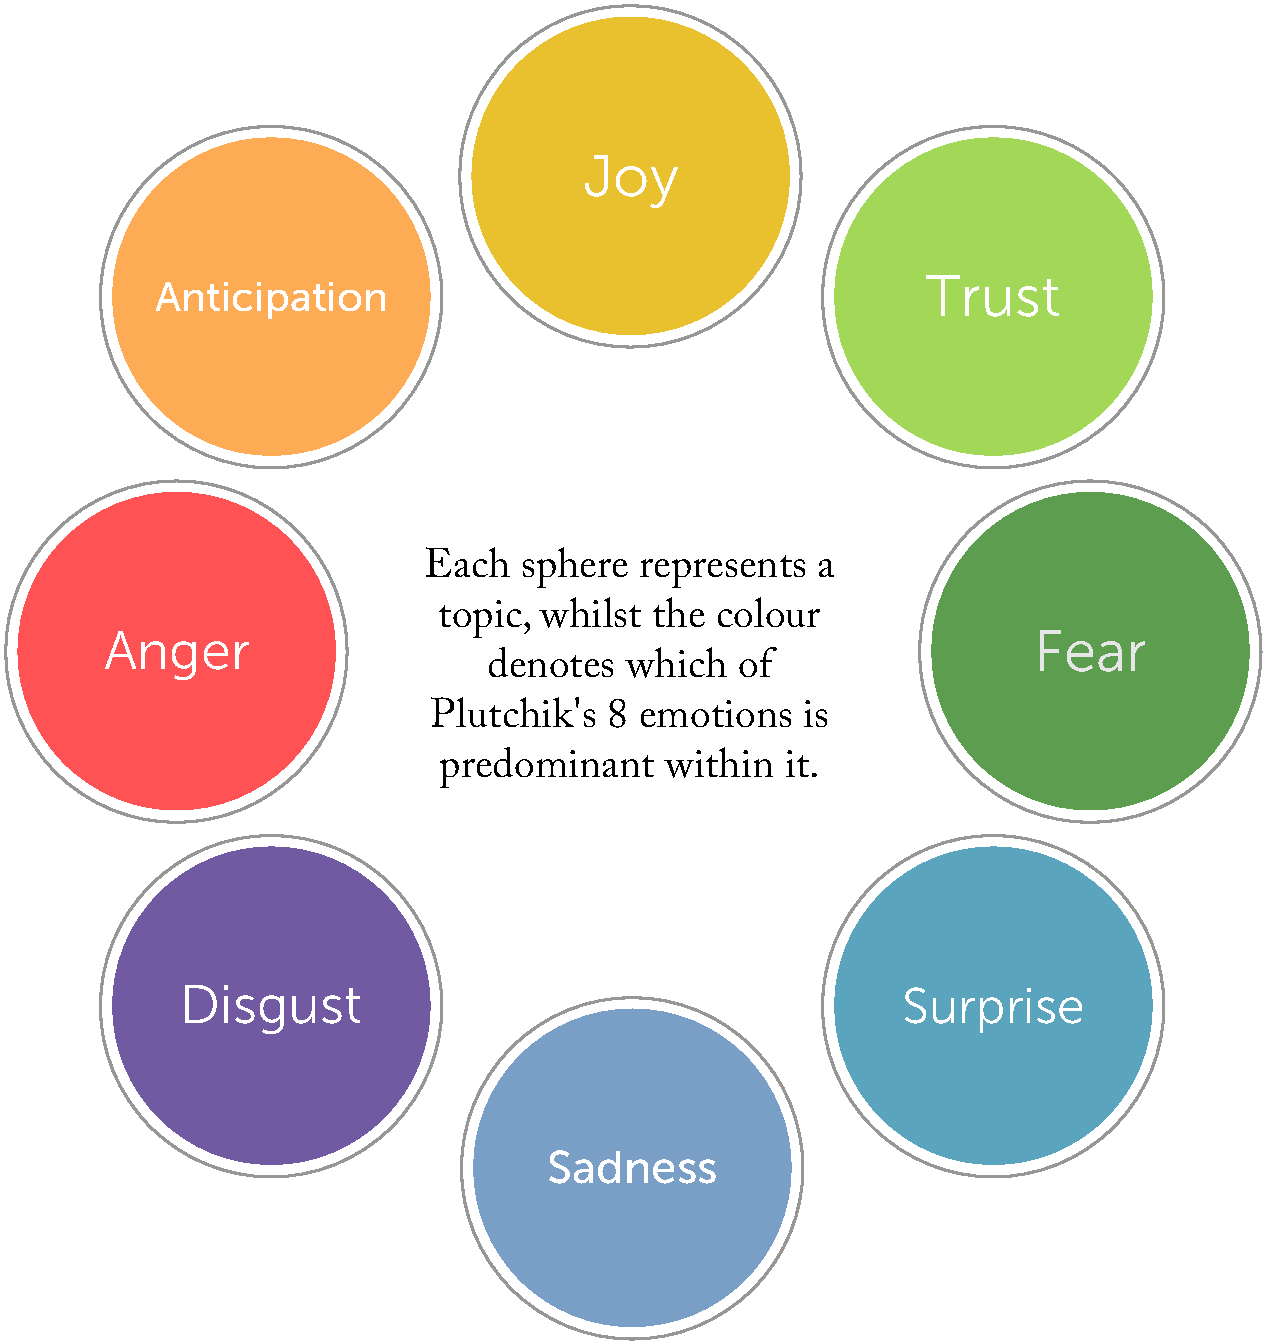
\includegraphics[width=0.9\textwidth]{figures/vis.pdf}
\end{figure}


\section{Evalutation}

We felt that both our web service implementation and visualisation tool met the project's core aims. 

Our classification service was simple to use for developers, and managed to mask the complexities of the underlying task well. Similarly, our results service proved effective and it's ability to easily filter results made it a viable data source for developers. The results for both services are returned in a simple and open format, thus further helping developers to make use of our engine and results. In developing our visualisation tool, we found that both services' fast response time made them viable tools for use within real-time data processing applications.

Our visualisation tool provided a simple intuitive interface for understanding sentiment on Twitter. In using HTML5 as a platform for delivery we ensured that our visualisation could be easily accessed by all across a wide variety of platforms.